\documentclass[a4paper,12pt]{article} %style de document
\usepackage[utf8]{inputenc} %encodage des caractères
\usepackage[french]{babel} %paquet de langue français
\usepackage[T1]{fontenc} %encodage de la police
\usepackage{times}
\usepackage[top=2cm,bottom=2cm,left=2cm,right=2cm]{geometry} %marges
\usepackage{graphicx} %'affichage des images
\usepackage{enumitem}
\usepackage{hyperref}
\usepackage{fancyhdr}
\pagestyle{fancy}
\usepackage{amssymb}
\usepackage[useregional]{datetime2}
\usepackage{datetime}
\usepackage{listings}
\newdateformat{monthyeardate}

\renewcommand{\footrulewidth}{1pt}
\fancyfoot[R]{\textbf{page \thepage}}
\fancyfoot[C]{}
\fancyfoot[L]{Dans le cadre de l'évaluation Licence 1 Informatique}
\renewcommand{\headrulewidth}{0pt}

\usepackage{verbatim}

\author{Guillaume LEMONNIER / Ronan CARRE\\Aboubacar KEITA / Alexis SUARD\\L1 info, 2020-2021\\Groupe 4A}

\title{Sokoban\\Projet Conception Logicielle}

\begin{document}

\maketitle

Le jeu Sokoban est un jeu de déplacement de caisse vers un point donné.
Le but est d'amener toutes les caisses sur des cibles afin de terminé le niveau.

\tableofcontents

\newpage

\section{Initialisation du Projet}

\subsection{Première approche}

En première approche nous avions envisagé de créer une map avec tableau de valeur en python.
Dans ce tableau il y aurait alors eu le joueur représenté par une valeur en charactère ou numéralle.
Chaque déplacement de l'utilisateur aurais alors changer la valeur de sa postion par une valeur de vide et changer la valeur de la case ou il souhaitais aller.
Il s'agissait alors d'une bonne approche pour le côté humain néanmois elle était veine et innutillle pour l'IA.

\newpage

\section{Vision du Projet}

\subsection{Les fonctions codés}

Le jeu se divise en trois phases clés.
La première phase se déroule lors du lancement de l'exécution du programme.
Cette phase demande à l'utilisateur de sélectionner le niveau désiré à l'aide des flèches directionnelles.
La deuxième phase s'occupe de l'exécution du jeu de son début jusqu'à une victoire.
Enfin la dernière phase est celle qui s'occupe de demander à l'utilisateur s'il souhaite relancer un niveau ou s'il souhaite quitter le jeu.

En parallèle à l'exécution du joueur une IA s'exécute  sur le coté droit, afin de mettre en compétition l'IA et le joueur.

\subsection{Répartition du travail}

Dans notre groupe de quatre nous nous sommes répartie le travail de manière suivante : 

Guillaume s'est occupé de la partie jeu du code, car ce dernier, sur son temps personnel, avais codé des petits jeux avec pygame lui procurant alors une plus grande aisance dans l'utilisation de cette librairie.
De plus Guillaume a participé à l'écriture du LaTex.

Ronan, quand à lui, s'est occupé de coder l'IA avec l'algorithme A* car il se sentais inspiré pour codé l'IA.
De plus il a écrit le Beamer pour la présentation orale et à aussi crée des maps pour le jeu en XSB.

Aboubacar s'est occupé d'une partie de l'algorithme A* avec Ronan et aussi d'une partie de la rédation du LaTex avec Guillaume.

Alexis à créé une parie des maps du jeu en XSB.

\newpage

\section{Developpement du code}

\subsection{Description des structures de données}

Le développement du jeu Sokoban comprend de nombreuses structures de données.
En effet celui-ci comporte six structures de données sans compter celles dans le code de l'IA.
Chaque page de code comprend une structure de donnée hormis le fichier lancement.py qui lui s'occupe uniquement de lancer l'execution, servir de centralisation des données et de décider quel partie du programme sera joué.

\subsubsection{Matrice}

La première structure de donnée à être utilisé est aussi la plus importante du jeu.
Il s'agit de la structure de la Matrix.py.
Cette dernière est composé de tous les éléments nécessaire afin de placer le joueur sur la matrice.
La class Matrice contient aussi la fonction move qui est la fonction la plus importante du jeu, en effet elle permet de tester si le déplacement est possible et si le jeu doit déplacer une caisse ou non.

\begin{lstlisting}
fonction move:
    copie <- classe
    test_direction <- position + direction_voulue
    si le joueur ne va pas dans le mur:
        si le joueur pousse une caisse:
            si le joueur ne pousse pas la caisse dans le mur:
                si le joueur ne pousse pas la caisse dans une caisse:
                    recherhce de la caisse qui va etre pousser : {...}
                        la pousser
                sinon:
                    ne pas avancer et retouner la copie
            sinon:
                ne pas avancer et retouner la copie
        deplacer la position du joueur
        placer les caisse sur la map vierge
        placer le joueur sur la map vierge
        deplacement + 1
        retourner la copie
    sinon:
        ne pas avancer et retouner la copie
\end{lstlisting}

Ainsi montrer la fonction move sert à la fois à faire le teste de possibilité et son déplacement si possible.
La classe Matrice comptient aussi la fonction victory testant si le joueur a réussi à bien placer toutes les caisses.
De ce fait la focntion teste si la coordonnée de chaque caisse correspond à la coordonnée d'une balise (étant donné que les caisse ne peuvent pas se mettre l'une sur l'autre elles auront toutes une coordonnée différente).
Si la coordonnée d'une caisse correspond à la coordonnée d'une balise alors le nombre de caisse bien placé augmente de un.
Enfin si la valeur de la variable des caisses bien placé correspond à la longueur de la liste des caisse alors c'est une victoire.

\subsubsection{Chose Level}

La deuxième classe la plus importante est la classe Chose level de chose level.py.
Cette classe s'occupe de en premier lieu de tester la valeur du niveau choisie dans sa fonction selection.
Si le niveau choisie est 0 alors le niveau choisie sera aléatoire sinon le niveau choisie sera le valeur entrée.

La deuxième fonction est la plus importante, en effet la fonction update ouvre d'abord le fichier XSB lié à la valeur du niveau choisi.
Puis une fois cela fait la fonction prend chaque ligne du XSB et l'ajoute à une liste qui viens d'être créé et chaque valeur de chaque ligne est un élément de la liste des lignes.
Ensuite la fonction teste la liste pour touver ou se situe le charactère 'p' afin de touver la valeur en y du personnage et ensuite elle cherche le deuxième 'p' afin de créer la coordonnée en x (programme uniquement possible en Python en effet l'avantage du python est qu'il est possible de mélanger les char et int afin de transformer le char '1' en int (1)).
Ensuite le programme fais la même chose pour les caisse à un détaille pret que pour les caisse il ne s'agit pas du charactère 'p' qui est cherché mais le charactère 'c'. 

\subsubsection{Les Run}

La troisième partie du code la plus importante est la partie des run.
Ces paties étaient à la base dans lancement.py mais se sont retrouvé dans des partie différentes afin de facilité la lecture et la compréhension de lancement.py.

La première est la classe Run Level du fichier run level.py.
Cette classe sert à tester la touche sur laquelle l'utilisateur appuye afin de déterminé si l'utilisateur veux selectionner le niveau supérieur ou alors le niveau inférieur.
De plus cette fonction sert à envoyer la commande de création du niveau dans chose level.py.
Enfin cette fonction affiche le niveau qui est actuellement pointé par l'utilisateur.

La deuxième est la classe Run de run.py.
Cette classe sert à tester la fleche sur laquelle l'utilisateur appuye pendant l'état de jeu et en fonction de la touche appuyer cette classe renvoie soit None (absence de touche) ou une liste de deux valeur (-1, 0 ou 1) en fonction de la touche appuyer.
Cette valeur est ensuite envoyé dans move de Matrix.py pour tenté de déplacé le personnage et/ou une caisse.

La dernière classe est la classe Win de run victory.py.
Cette classe se lance uniquement si l'utilisateur gagne.
Elle sert donc à demander si l'utilisateur souhaite relancer un niveau ou s'il souhaite arréter de jouer.
Si l'utilisateur choisi d'arréter de joué alors la boucle while s'arrète et la jeu se ferme avant de terminé le programme.
Et si l'utilisateur choisi de continué de joué le programme créer une nouvelle Matrice afin de recommancer une partie de zéro.

\subsubsection{Visuel}

La dernière classe est la classe Visuel de visuel.py.
Cette classe se sert de la Matrice qui lui est arrivé en entrée pour en sortir l'élément grille afin d'avoir accès à la liste pour en construire une représentation dans le screen.
Pour chaque élément de la liste il y a un élément visuel relié.
Ainsi en fonction du charactère entrée le code choisira tel ou tel tuile pour le représenté.

\subsection{Description de l'algorithme A*}

\newpage

\section{Construction du Projet}

\subsection{Schéma du projet}

\setlength{\unitlength}{1mm}
\begin{picture}(40,20)

\put(55,0)
{
    \framebox(40, 20){lancement.py}
}
\put(75, -20)
{
    \framebox(0, 20){}
}
\put(35, -20)
{
    \framebox(80, 0){}
}
\put(5, -30)
{
    \framebox(30, 20){visuel.py}
}
\put(75, -30)
{
    \framebox(0, 10){}
}
\put(60, -50)
{
    \framebox(30, 20){matrix.py}
}
\put(50, -60)
{
    \framebox(0, 40){}
}
\put(30, -80)
{
    \framebox(30, 20){AI.py}
}
\put(75, -100)
{
    \framebox(0, 50){}
}
\put(60, -120)
{
    \framebox(30, 20){chose level.py}
}
\put(115, -60)
{
    \framebox(0, 40){}
}
\put(95, -60)
{
    \framebox(40, 0){}
}
\put(95, -70)
{
    \framebox(0, 10){}
}
\put(115, -70)
{
    \framebox(0, 10){}
}
\put(135, -70)
{
    \framebox(0, 10){}
}
\put(80, -90)
{
    \framebox(25, 20){run level.py}
}
\put(120, -90)
{
    \framebox(30, 20){run victory.py}
}
\put(105, -90)
{
    \framebox(15, 20){run.py}
}
\end{picture}

\newpage

\subsection{Chaîne de traitement}

Le projet commence en éxécutant la commande python3 lancement.py.
Ce fichier contient la fonction while qui s'occupe de faire tourner le jeu continuellement tant que l'utilisateur n'a pas demandé de fermer le jeu.
Ce fichier sert de hub (point de ralliment) pour toutes les fonction.
Ainsi le lancement.py est le fichier principale mais n'est pas celui contenant les fonctions les plus importantes.
lancement.py vérifie les états de jeu de matrix.py afin de savoir dans quel situation de jeu le joueur se trouve.
Si l'état de Matrice.level running est à true, alors le code execution la class run level afin de demandé à l'utilisateur de selectionné un niveau.
Si l'état de Matrice.victoire est à true alors le programme lance run victory afin de demander à l'utiisateur s'il veut rejouer.
Enfin si les deux test sont à false alors la Matrice s'initialise lors du premier tour de boucle puis attend une action du joueur. 

Le code de lancement.py entre donc dans matrix.py pour y effectué des tests d'états afin de choisir quel run exécuter.
Mais le code de matrix.py ne sert pas qu'à vérifié des états il sert aussi à executer le code de chose level.py afin de lancer un niveau à créer et de récupérer ses données.

Le code de chose level.py sert à ouvrir le fichier XSB selectionné et à le transformer en plusieur listes.
Le fichier matrix.py à alors juste à se servir sur les listes créer par le fichier chose level.py.

Enfin la liste de matrix.py sort à chaque action pour aller dans le lancement.py puis dans visuel.py afin d'y être analysé pour en sortir un affichage pour l'utilisateur.

\newpage

\section{Mise en fonctionnement}

La mise en fonctionnement est en trois phases comme le code.
Les phases sont indépendantes et ont un style graphics commun avec la police de l'écriture et part leurs positionnement.

\subsection{Côté utilisateur}

\subsubsection{Démarrage}

Le jeu commence par la première phase.
Cette phase est la phase de selection du niveau.
Il est simplement représenté par une phrase demandant quel niveau l'utilisateur souhaite éxécuter ainsi que le niveau qui est actuellement ciblé.

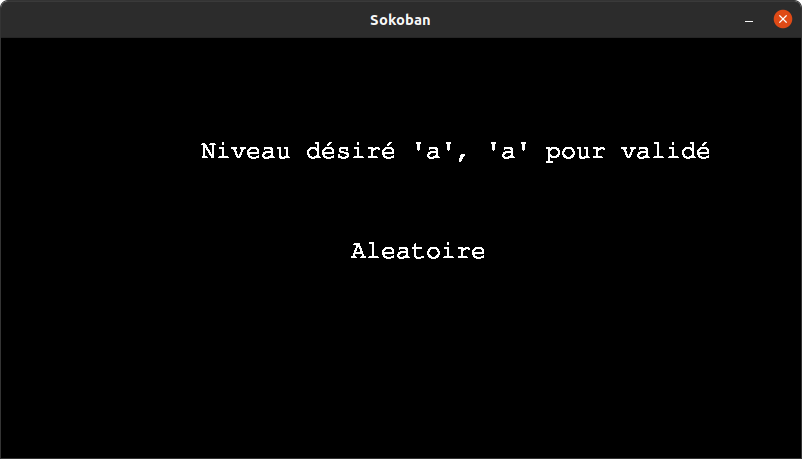
\includegraphics[scale = 0.25]{../picture/starting.png}
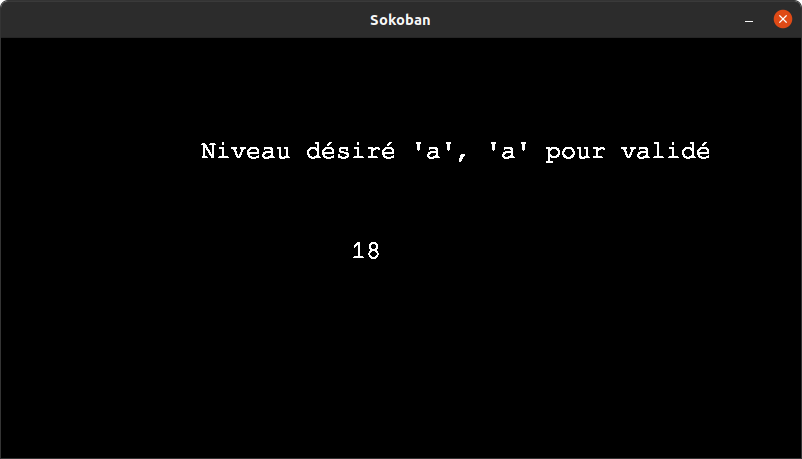
\includegraphics[scale = 0.25]{../picture/starting2.png}

L'utilisateur a alors uniquement la possibilité de naviguer à gauche ou à droite avec les fleches afin de selectionner le niveau.
Une fois qu'il à décidé du niveau voulu il n'a plus qu'à faire un double 'a'.

\subsubsection{Phase de Jeu}

La phase de jeu succede la phase de choix du niveau.
Lors de cette phase le joueur à la possibilité de se mouvoir sur deux axes et donc dans quatre directions.
Il a aussi la possibilité de pousser des caisses mais pas de les tirer.

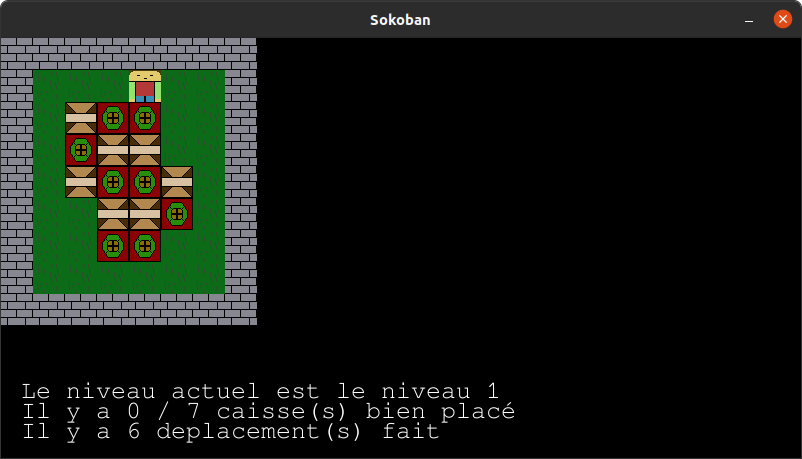
\includegraphics[scale = 0.25]{../picture/game1.png}
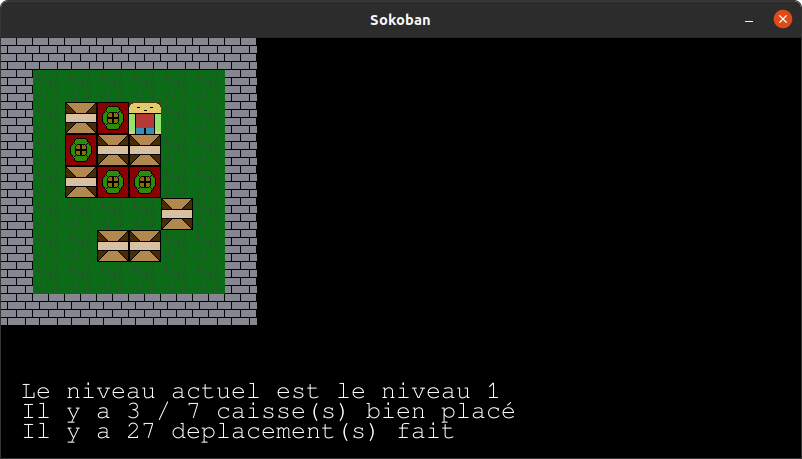
\includegraphics[scale = 0.25]{../picture/game2.png}

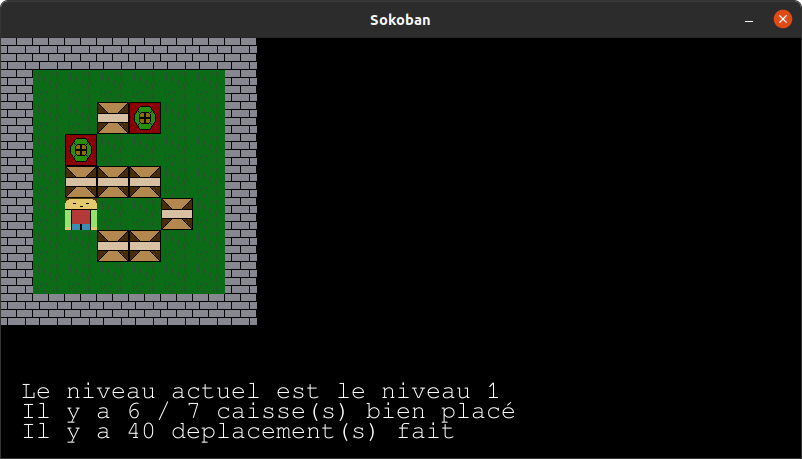
\includegraphics[scale = 0.25]{../picture/game3.png}

Les caisses sont représenté par le dessin suivant 
\includegraphics{../picture/caisse.png}

Le personnage est représenté par le dessin suivant
\includegraphics{../picture/heros.png}

Les murs sont représenté par le dessin suivant 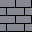
\includegraphics{../picture/mur.png}

Les cible sont représenté par le dessin suivant 
\includegraphics{../picture/ciblage_tro-oof.png}

Enfin les zones vides sont représenté par de l'herbe 
\includegraphics{../picture/weed.png}

Cette représentation est liée à la grille qui est envoyé dans la fonction update de visuel.py.
Chaque représenation visuel est indépendante et redessine intégrallement la fenêtre lors d'une action.


\subsection{Côté A*}

\newpage

\section{Conclusion}

\subsection{Résumé de la conception}

La conception du jeu à été entièrement réalisé par Guillaume LEMONNIER.
Bien qu'au départ il y eu une répartition du travail de manière homogène, l'absentéhisme due au confinement, à changer les rôles et à changer la répartition du travail.
Quand à l'IA, elle a été entièrement réalisé par Ronan CARRE pour mêmes raisons qui ont poussé Guillaume LEMONNIER à réalisé seul le jeu.

Le jeu se déroule en trois phases.
La phase de selection de niveau.
La phase d'éxécution du niveau.
Et la phase de relancement ou non du jeu.

L'IA quand à elle 

\subsection{Pour aller plus loin}

Pour aller pour loin nous avons penssé à plusieurs améliorations tels que ajouter du sound design.
Afin de rendre le jeu plus vivant et réaliste pour l'utilisateur.
Nous avions aussi pensé à ajouter des animation de déplacement pour l'utilisateur, afin de rendre le jeu moins rigide visuellement mais toujours utilisable pour l'IA.
Enfin nous avons pensé à créer une nouvelle phase du jeu, en parralèle de l'execution de niveeau, un mode de création de niveau à la sourie avec les blocs sur le côté.
Le joueur aurais alors uniquement à selectionner une case pour en faire un élément.
Suite à sa conception le niveau serait enregistré en XSB et tester par l'IA pour vérifié sa faisabilité.

\end{document}